% SPDX-License-Identifier: CC-BY-4.0
% Copyright (c) 2026 Jonathan Yantis. Research draft; not submitted.
\documentclass[11pt,letterpaper]{article}
\usepackage[margin=0.85in]{geometry}
\usepackage[T1]{fontenc}
\usepackage{mathptmx,amsmath,amssymb,booktabs,array,ragged2e,xcolor,microtype,xurl,hyperref,fancyhdr,tikz,pgfplots}
\usetikzlibrary{arrows.meta,positioning}
\pgfplotsset{compat=1.18}
\definecolor{studyblue}{RGB}{39,83,109}
\definecolor{studyorange}{RGB}{173,90,35}
\hypersetup{colorlinks=true,urlcolor=studyblue,citecolor=studyblue,linkcolor=black,pdfauthor={Jonathan Yantis},pdftitle={A Shared Time Base for Indoor PNT: PToB Sensor Fusion, Selective UWB Augmentation, and a Validation Programme}}
\setlength{\parindent}{1em}\setlength{\parskip}{3pt}\setlength{\headheight}{14pt}\setlength{\emergencystretch}{2em}
\widowpenalty=10000\clubpenalty=10000
\pagestyle{fancy}\fancyhf{}\fancyhead[L]{\small PToB and Indoor PNT}\fancyhead[R]{\small Review draft, 26 October 2026}\fancyfoot[C]{\small\thepage}
\newcolumntype{L}[1]{>{\RaggedRight\arraybackslash}p{#1}}
\newcommand{\ns}{\,\mathrm{ns}}\newcommand{\us}{\,\mu\mathrm{s}}\newcommand{\ms}{\,\mathrm{ms}}
\newcommand{\code}[1]{\texttt{#1}}
\begin{document}
\title{\vspace{-1.3em}A Shared Time Base for Indoor PNT\\[5pt]\large PToB Sensor Fusion, Selective UWB Augmentation,\\and a Validation Programme}
\author{Jonathan Yantis}
\date{26 October 2026\\\small Research draft prepared for author review; publication approval pending}
\maketitle
\begin{abstract}
Indoor positioning, navigation and timing (PNT) must combine observations made by heterogeneous sensors despite occlusion, multipath, drifting clocks and intermittent connectivity. We investigate Precision Time over BLE (PToB) as a common event-time service beneath an indoor navigation network. The proposed architecture combines inexpensive inertial, wheel, pressure, magnetic, acoustic and visual observations with selectively deployed ultra-wideband (UWB), Bluetooth ranging or surveyed landmarks. Existing PToB evidence motivates this direction: a dated W12 population has 60.328 ns bias-inclusive relative-PPS RMS across 522 eligible of 600 logged observations; its complete second 300-second window has 38.312 ns RMS. These finite source-relative observations do not establish calibrated UTC accuracy, GNSS time-transfer equivalence, or indoor position accuracy. We derive separate sensor-motion and radio-propagation budgets, a causal timestamp and cross-clock contract, correlated clock-error treatment, observability requirements and holdover limits. A two-layer design uses PToB for event alignment and orchestration while retaining independently qualified ranging clocks where needed. Reproducible analytical examples, a cost sensitivity model and a falsifiable indoor evaluation programme define what would establish practical benefit. No new localization experiment, UWB integration or hardware qualification is claimed.
\end{abstract}
\noindent\small Copyright \copyright\ 2026 Jonathan Yantis. Manuscript and original vector figures: \href{https://creativecommons.org/licenses/by/4.0/}{CC BY 4.0}. Verification code and ordinary documentation: MIT.\normalsize

\section{Motivation and research question}
A building may already contain cameras, environmental sensors, BLE devices and mobile instruments. Their observations become more useful for navigation when they identify the same time and place. An inertial measurement can propagate a pose between landmark updates; pressure can suggest a floor transition; a surveyed range can restrain drift. Combining them requires knowing when each physical observation occurred, which spatial frame it belongs to, and whether its timing and measurement quality remain valid.

PToB develops shared time over BLE periodic advertising, with causal clock maps, explicit source ancestry and finite validity \cite{viability,implementation}. The research question is whether a reusable timing layer can reduce integration cost and improve indoor estimation across sensor types. Our contribution is a proposed architecture and quantitative research plan, supported by existing timing evidence and analytical examples. All numerical navigation requirements below are candidate study assumptions. The latest discussed public hardware collection is dated 24 October 2026; external primary sources were reviewed on 26 October. This manuscript adds no physical measurement.

\newpage
\section{What the timing evidence establishes}\label{sec:evidence}
\subsection{Use the latest public population without erasing its failures}
Table~\ref{tab:evidence} separates the selected post-repair W12 observations from earlier experiments. A residual is the delivered clock coordinate evaluated at a captured reference PPS, relative to the stated reference path; it is not a measurement of every electrical sensor output. Let $\mathcal E$ be the eligible set. We report
\begin{equation}
 \bar e=\frac{1}{n}\sum_{k\in\mathcal E}e_k,\quad
 e_{\rm RMS}=\sqrt{\frac{1}{n}\sum_{k\in\mathcal E}e_k^2},\quad
 s=\sqrt{\frac{1}{n}\sum_{k\in\mathcal E}(e_k-\bar e)^2},\qquad n=|\mathcal E|.
\end{equation}
Thus $e_{\rm RMS}^2=\bar e^2+s^2$. RMS includes bias; a mean, centered spread and RMS are different statistics. We do not average unlike RMS populations into a single headline precision.

\begin{table}[ht]\centering\small
\caption{Separate historical relative-timing populations; all eligible tails retained. The stable W12 row is a subset of the preceding row.}\label{tab:evidence}
\begin{tabular}{@{}L{61mm}rrr@{}}\toprule
Population & Eligible / total & RMS ns & Max $|e|$ ns\\\midrule
24 Oct W12, two 300 s windows &522 / 600&60.328&180\\
\quad W12 second-window subset &300 / 300&38.312&121\\
24 Oct downstream T096 &451 / 600&61.922&211\\
24 Oct selected TX at downstream RX &58 / 120&108.306&226\\
22 Oct N30 fixed window &657 / 660&166.590&1591\\
22 Oct fresh second-board transfer &48 / 64&150.954&362\\
12 Oct V14 reference-valid causal &436 / 602&62.504&191\\\bottomrule
\end{tabular}
\end{table}

The W12 experiment followed a declared 120-second warmup. W12 0.2.10 and T096 0.15.169 used frozen receive/relay adjustments. The GNSS witness did not train the BLE discipline. Of 600 W12 records, 78 were source-unavailable; 522 eligible phases had mean $+40.695\ns$. The complete second window had mean $+20.737\ns$. Downstream records retain 109 no-map, 36 expired and four reference-ineligible cases. Selected TX retains 61 missing follow-up matches and one missing PPS bracket. These received-path TX observations do not isolate physical transmitter delay \cite{w12}.

The 22 October N30 window retains three invalid records, zero nominal missing and a 1591 ns tail. The later transfer retains 16 invalid records. Its offset was selected using the earlier completed window, so that window cannot also validate the new offset \cite{fine}. V14 retains 65 invalid-reference, three expired and 98 unobserved opportunities. Its 501 all-causal samples, including invalid references, have 3.929 ms RMS; the maximum witness gap is 59.017 s \cite{v14}. These are distinct source versions, paths and populations, not a controlled platform ranking.

\subsection{The GNSS comparison requires a defined endpoint and uncertainty}
NIST describes well-designed one-way GNSS timing at better than 100 ns after minutes and about $\pm10\ns$ with a 24-hour average and good local clock \cite{gnssone}. It describes common-view transfers typically at 1--10 ns \cite{gnsscommon}. Those examples differ in calibration, averaging and reference. Tens-of-nanoseconds relative RMS in PToB therefore motivates comparison with some GNSS timing applications, but establishes no equivalence. A matched comparison needs the same endpoint, duration, bandwidth, availability and independently measured uncertainty. RF detector, antenna, cable, GPIO and reference delays, physical output timing and absolute UTC association remain unqualified here. Checksums establish record identity, not accuracy.

\section{Two timing budgets: moving sensors and propagating waves}\label{sec:budgets}
\subsection{Sensor alignment follows motion speed}
For a sensor offset $\delta t$ and bounded platform speed $v_{\max}$ and acceleration $a_{\max}$, a local temporal contribution to position error satisfies
\begin{equation}
 E_{p,t}\leq v_{\max}E_t+\tfrac12 a_{\max}E_t^2,
 \qquad E_{\theta,t}\leq\omega_{\max}E_t.\label{eq:motion}
\end{equation}
At an assumed $2\,\mathrm{m/s}$, $1\ms$ contributes 2 mm at constant speed; $100\ns$ contributes $0.0002\,\mathrm{mm}$. At $180^\circ/\mathrm{s}$, $1\ms$ contributes $0.18^\circ$; at a one-metre lever arm this is approximately 3.142 mm transverse error. Reducing temporal misalignment may help rapid motion and multi-sensor consistency. Once clock error is small, exposure, readout, digital filtering, scan timing and extrinsic calibration can dominate. A better network clock cannot identify an undocumented sensor delay.

\subsection{Radio ranging follows propagation speed}
For one-way free-space propagation, with $c=299\,792\,458\,\mathrm{m/s}$,
\begin{equation}
 \delta d=c\,\delta t,\qquad E_t=E_d/c.\label{eq:light}
\end{equation}
A 100 ns differential timestamp error corresponds to 29.979 m of range-difference error. Allocating 0.10 m to that error alone allows approximately 333.564 ps; 1 m allows 3.336 ns. Position error also depends on geometry, NLOS bias and antenna calibration. These conversions are not position predictions, and a one-way expression must not silently become the half-round-trip expression for two-way ranging.

\begin{table}[ht]\centering\small
\caption{Analytical sensitivity to the same time error. Radio column is one-way range or range difference; motion column assumes $2\,\mathrm{m/s}$. These are not measured navigation results.}
\begin{tabular}{@{}rrr@{}}\toprule
Time error & Motion contribution, mm & Radio contribution, m\\\midrule
100 ps &0.0000002&0.029979\\
1 ns &0.000002&0.299792\\
100 ns &0.0002&29.979246\\
1 $\mu$s &0.002&299.792458\\
1 ms &2&299792.458\\\bottomrule\end{tabular}
\end{table}

PToB's published residuals are not measurements of differential UWB anchor-clock error. Even using 60.328 ns as a purely illustrative differential error would imply approximately 18.086 m of range difference. We therefore propose \emph{shared event time plus a separately qualified fine-ranging layer}. Current evidence supports investigating event alignment and scheduling first, rather than assigning PToB sole responsibility for centimetre TDoA.

\subsection{Indoor propagation also affects the timing layer}
An unmodelled 30 m radio path contributes approximately 100.069 ns. In a one-way time-transfer link, observation of clock offset and path delay is intrinsically coupled unless geometry or another constraint separates them. A calibration at one position may absorb its propagation delay and fail when a tag moves. Surveyed infrastructure can supply nominal path corrections; mobile links need range-informed correction or an explicit changing-delay allowance. Multipath adds an unknown excess path. NIST's indoor UWB measurements show why connectivity alone does not guarantee precise direct-path ranging \cite{nistindoor}.

\section{Proposed unified sensor-network architecture}\label{sec:architecture}
\begin{figure}[ht]\centering
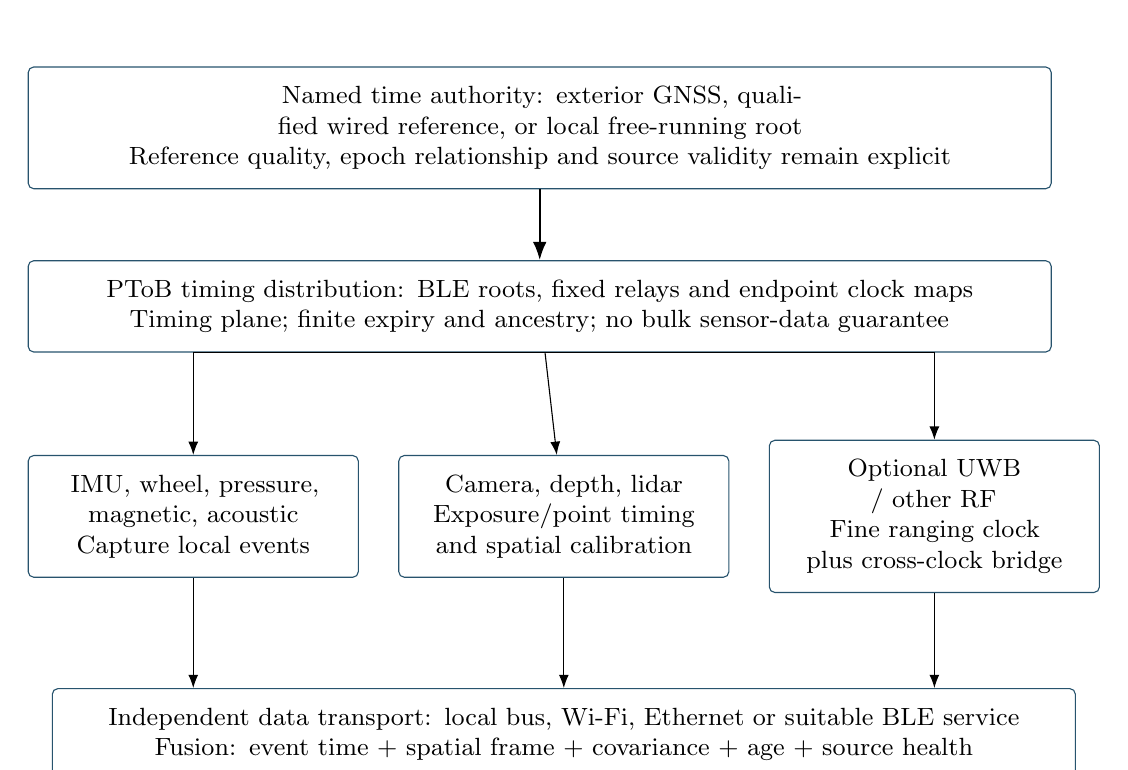
\begin{tikzpicture}[>=Latex,box/.style={draw=studyblue,rounded corners=2pt,align=center,font=\small,inner sep=7pt},node distance=9mm]
\node[box,text width=125mm](root){Named time authority: exterior GNSS, qualified wired reference, or local free-running root\\Reference quality, epoch relationship and source validity remain explicit};
\node[box,text width=125mm,below=of root](mesh){PToB timing distribution: BLE roots, fixed relays and endpoint clock maps\\Timing plane; finite expiry and ancestry; no bulk sensor-data guarantee};
\node[box,text width=37mm,below=13mm of mesh.south west,anchor=north west](cheap){IMU, wheel, pressure,\\magnetic, acoustic\\Capture local events};
\node[box,text width=37mm,right=5mm of cheap](vision){Camera, depth, lidar\\Exposure/point timing\\and spatial calibration};
\node[box,text width=37mm,right=5mm of vision](uwb){Optional UWB / other RF\\Fine ranging clock\\plus cross-clock bridge};
\node[box,text width=125mm,below=14mm of vision](fusion){Independent data transport: local bus, Wi-Fi, Ethernet or suitable BLE service\\Fusion: event time + spatial frame + covariance + age + source health};
\draw[->,thick](root)--(mesh);
\draw[->](mesh.south)-|(cheap.north);\draw[->](mesh)--(vision);\draw[->](mesh.south)-|(uwb.north);
\draw[->](cheap.south)--(cheap.south |- fusion.north);\draw[->](vision)--(fusion);\draw[->](uwb.south)--(uwb.south |- fusion.north);
\end{tikzpicture}
\caption{Proposed architecture. Every sensor adapter, localization estimator and UWB bridge in this figure is future integration work. A local root can support relative navigation without a UTC claim.}\label{fig:architecture}
\end{figure}

\subsection{A common contract across heterogeneous devices}
The fixed infrastructure distributes a named time domain and surveyed spatial frame. Mobile nodes capture local events, use valid maps to attach shared event time, and transmit measurements with their quality and identity. A navigation consumer can be on the tag, a local gateway or both. Sensor payloads need not traverse the timing mesh. Low timing traffic does not imply that camera streams fit in BLE periodic advertisements.

The root may reference exterior GNSS through a measured ingress path, a qualified wired source, or a local oscillator. Losing UTC need not destroy local relative-time utility; losing a valid inter-node relationship must invalidate cross-node comparisons. Root changes require measured continuity or a new domain relationship. A root identity alone cannot justify joining epochs across resets. The proposed contract records source ancestry to identify common failures, rather than treating multiple descendants as independent time references.

Current target roles remain as documented in their own firmware guides. T096 GM/RC and separate DC images are distinct; W12, SS3 and N30 names do not imply GNSS, GM capability or UWB support. The paper proposes adapters, without modifying firmware or its role authority. The existing gPTP/robotics study discusses a possible wired-time ingress separately \cite{robotics}.

\subsection{Navigation services beyond a position dot}
Useful outputs include timestamped pose and velocity, heading, floor hypotheses, anchor/landmark observations, map-frame transforms and uncertainty. Route guidance additionally needs a traversable map and access constraints. Dead reckoning propagates between observations; globally referenced landmarks constrain accumulated drift. A network that distributes time only has not yet provided these navigation services.

\section{Timestamp semantics and a causal clock bridge}\label{sec:contract}
\subsection{Timestamp the measurement event}
An IMU timestamp should identify its effective sampling aperture or a measured data-ready relationship, not just SPI completion. A camera needs exposure timing and, when relevant, per-row readout; a spinning lidar needs per-point time. Pressure and magnetic sensors need integration/filter-delay metadata. Acoustic observations need sample-clock and microphone-delay knowledge. A receiver callback is a transport event until its relationship to acquisition has been established. Temporal calibration has a substantial history: Qin and Shen jointly estimate camera--IMU time offset in visual-inertial estimation \cite{qin}; Kalibr documents spatial and temporal camera--IMU calibration and separate intrinsic/noise prerequisites \cite{kalibr}. Shared network time reduces one uncertainty source while leaving device calibration necessary.

\begin{table}[ht]\centering\small
\caption{Proposed logical record contract; no new wire profile or implemented API is asserted. Fields may be referenced through immutable metadata rather than repeated in each sample.}
\begin{tabular}{@{}L{37mm}L{112mm}@{}}\toprule
Record group & Required meaning\\\midrule
Event identity &Sensor identity, boot/counter incarnation, sequence, raw latch, event definition and sensor settings. Preserve reset/wrap and dropped-sample indicators.\\\addlinespace
Time mapping &Domain and epoch, map version, event-time coordinate, map activation and availability, original expiry and source ancestry; distinguish capture time from arrival time.\\\addlinespace
Timing quality &Measured residual statistic versus calibrated bound, bound scope/confidence if available, age, rate/holdover model, unresolved delay terms and UNKNOWN flags.\\\addlinespace
Spatial metadata &Frame/map revision, anchor or sensor extrinsics and uncertainty; surveyed versus estimated coordinates. An alias is not a survey.\\\addlinespace
Observation quality &Units, covariance and correlations, calibration revision, NLOS/occlusion indicators, processing delay, validity and reason.\\\addlinespace
Consumer status &Arrival time, current age, use/reject/degrade decision and reason. Retain unavailable or rejected observations in accounting.\\\bottomrule
\end{tabular}
\end{table}

\subsection{Map composition must preserve the clock and validity domains}
For local counter $q$, a causal affine map for segment $k$ is
\begin{equation}
 \hat T(q)=T_k+a_k(q-q_k),\qquad q\in I_k.\label{eq:map}
\end{equation}
Use integer/fixed-point epoch arithmetic and local differences to avoid losing nanoseconds in large floating-point civil epochs. Counter incarnation is part of the key. A sensor or UWB counter $u$ needs its own bridge, e.g.
\begin{equation}
 q=q_b+b(u-u_b),\qquad
 \hat T(u)=T_k+a_k\{q_b-q_k+b(u-u_b)\}.\label{eq:bridge}
\end{equation}
Each validity interval must be transformed into the same coordinate before intersection. For an online scored event, its map and all supporting references must have been available by the declared decision time. A later model may support retrospective analysis only if labelled as such. A fitted host-SPI read midpoint is not a physical UWB receive event. Prefer a qualified common trigger or hardware cross-capture; otherwise retain measured bracket/asymmetry uncertainty.

For small errors, an absolute event-time budget combines source, BLE transfer, cross-clock bridge, acquisition endpoint and sensor-delay terms. Their bounds add conservatively after conversion to common time units. Independent standard uncertainties may combine quadratically only with justified independence. An unknown term makes the claimed total bound unknown; a small empirical RMS cannot fill that gap.

\section{How UWB and other ranging technologies complement PToB}\label{sec:ranging}
\subsection{First integration: UWB two-way ranges on a common observation timeline}
Two-way ranging estimates flight time from local elapsed intervals, allowing a ranging exchange without globally aligned clock offsets. In an ideal rate-corrected single-sided exchange,
\begin{equation}
 \hat\tau=\tfrac12(R_A-D_B),\qquad \hat d=c\hat\tau,\label{eq:twr}
\end{equation}
where $R_A$ is A's round-trip interval and $D_B$ is B's turnaround interval expressed in A-compatible seconds. Subtracting raw ticks from unrelated oscillators is invalid. If the two clocks have fractional frequency errors $\epsilon_A,\epsilon_B$, a first-order contribution is
\begin{equation}
 \delta\tau\simeq\epsilon_A\tau+\tfrac12(\epsilon_A-\epsilon_B)D_B.
\end{equation}
At a hypothetical 1 ms turnaround and 1 ppm differential rate error, the second term alone is 0.5 ns, or approximately 0.150 m. Double-sided protocols mitigate such errors but still require proper timestamp and delay models. Rathje and Landsiedel analyze DS-TWR/DS-TDoA bias and variance under multipath and NLOS \cite{rathje}. NIST separately studies oscillator phase noise and temperature drift in UWB ranging \cite{hati}. PToB software time-map discipline is not RF oscillator or carrier-phase discipline.

The first proposed integration keeps UWB's native RF timestamps and ranging protocol intact. PToB labels the range's effective observation interval for IMU/vision fusion, coordinates coarse exchange slots and records source health. A moving tag requires the positions of the communicating antennas at the actual transmit/receive events or a bounded quasi-static approximation. A midpoint timestamp is an approximation whose error depends on motion and exchange duration. Bitcraze's published protocol index provides public examples of distinct TWR and TDoA implementations, not PToB interoperability \cite{bitcraze}.

\subsection{Later research: qualified TDoA fine synchronization}
For an uplink tag event received at surveyed anchors $i,j$, a simplified difference model is
\begin{equation}
 z_{ij}=\|p-a_i\|-\|p-a_j\|+c(\beta_i-\beta_j)
          +(\eta_i-\eta_j),\label{eq:tdoa}
\end{equation}
where $\beta_i$ is residual anchor time offset in seconds and $\eta_i$ includes range-equivalent detector, antenna, noise and multipath effects. A common tag transmit epoch cancels for the same event; different packets need a motion/transmit-time model. Centimetre or decimetre TDoA requires independently qualified differential anchor time at the necessary subnanosecond scale. Candidate solutions include a dedicated UWB synchronization protocol, wired common clock, or a measured joint clock/range estimator. PToB may give coarse epoch alignment and recovery assistance. No claim here substitutes present PToB PPS RMS for a fine UWB synchronization certificate.

\subsection{Additional modalities}
Bluetooth Channel Sounding supports phase-based ranging and round-trip timing, with application processing and support required in both controllers \cite{channelsounding}. It is a distinct feature from periodic advertising; existing PToB boards do not acquire it through a timestamp change. Direction finding, compatible Wi-Fi ranging and optical landmarks are additional candidate observations, each needing a device-specific measurement model. RSSI can supply proximity or fingerprint evidence without being treated as precise flight time. Acoustic ranging uses sound speed: at an assumed $343\,\mathrm{m/s}$, $100\us$ corresponds to 34.3 mm, but temperature, airflow, transducer delays and reverberation remain. Magnetic and pressure observations can aid heading/floor inference only with disturbance and ambiguity models. These are proposed integrations, without demonstrated compatibility or accuracy.

\section{Fusion, correlation and spatial observability}\label{sec:fusion}
\subsection{Estimate state at observation time}
A candidate estimator maintains pose, velocity and inertial biases, with selected clock and sensor-delay variables:
\begin{equation}
 x(t)=\{p(t),v(t),R(t),b_a(t),b_g(t),\beta_{1:m}(t),\dot\beta_{1:m}(t),d_{1:s}\}.
\end{equation}
Not every system needs every variable. Some may be calibrated constants with documented uncertainty. A sliding-window factor graph or filter can combine inertial propagation, ranges, visual bearings, wheel increments, pressure and landmarks. In a generic robust objective,
\begin{equation}
 \hat X=\arg\min_X\sum_{\ell}\rho_\ell\!\left(
    r_\ell(X,z_\ell)^{\mathsf T}\Sigma_\ell^{-1}r_\ell(X,z_\ell)\right),\label{eq:fusion}
\end{equation}
$\Sigma_\ell$ must include the applicable measurement and time uncertainty; correlated observations require joint residual blocks or explicit shared latent variables. Robust losses reduce influence under their model, but do not certify integrity or justify deleting failures from evaluation.

If an observation model is $h(x(t))$, local timing uncertainty $\delta t$ produces $r_t\simeq J_t\delta t$, with $J_t=\mathrm{d}h/\mathrm{d}t$. For independent zero-mean time error,
\begin{equation}
 \Sigma_{\rm effective}=\Sigma_z+J_t\sigma_t^2J_t^{\mathsf T}.\label{eq:cov}
\end{equation}
Biases, cross-covariances or an unknown timing bound require additional treatment. A stale measurement can be incorporated at its original event time with propagation to the current estimate; relabelling it with arrival time creates a different measurement. Out-of-sequence handling must be bounded by memory and latency policy.

\subsection{A common source creates correlated errors}
Write endpoint time error as $e_i=g+\ell_i$, with common source error $g$ and local error $\ell_i$. Simultaneous differences cancel $g$ only under that model. In general,
\begin{equation}
 \operatorname{Var}(e_i-e_j)=\sigma_i^2+\sigma_j^2-2\operatorname{Cov}(e_i,e_j).\label{eq:correlation}
\end{equation}
Independent equal 60 ns standard deviations give 84.853 ns differential standard deviation; correlation 0.9 gives 26.833 ns. These are hypothetical standard deviations, not the measured bias-inclusive RMS in Table~\ref{tab:evidence}. They show why single-node scores do not establish differential ranging performance. Root errors may cancel for simultaneous relative observations and remain in absolute UTC or measurements at different times. Shared reference, map and calibration dependencies must follow the observations into fusion.

\subsection{Time does not supply missing geometry}
A common clock supplies no anchor coordinates, absolute translation or heading. In 3D, range-only instantaneous positioning generally needs at least four suitably placed known anchors for an unambiguous solution, with additional redundancy desirable; minimum counts alone do not guarantee uniqueness. TDoA needs enough independent differences and suitable geometry. Coplanar or corridor layouts can leave height or along-track error poorly constrained. IMU-only motion drifts; monocular geometry has scale/frame ambiguities unless additional observations resolve them. Pressure suggests relative height under environmental assumptions, not a guaranteed floor label.

With local range Jacobian $H$ and covariance $\Sigma$, an illustrative linear covariance is $(H^{\mathsf T}\Sigma^{-1}H)^{-1}$ only when the system is full rank and its model is appropriate. Survey uncertainty, correlated NLOS bias and clock/position coupling must be retained. A map or motion prior can improve a solution while concealing a weak measurement geometry; evaluation should expose that dependence.

\section{Deployment, availability and resource budgets}\label{sec:deployment}
\subsection{Start with a fixed surveyed backbone}
A candidate installation uses fixed timing relays where possible, heterogeneous tags and selected ranging/visual landmarks at difficult transitions. Anchor coordinates, height diversity and frame transforms are surveyed independently. Site design considers metal, walls, people, moving doors and RF coexistence. The initial pilot evaluates one-hop and one-relay paths separately. Greater hop counts, mobile parents and inter-floor handover require their own populations; they are not established by current evidence.

A root failover may change phase, delay or ancestry. Consumers preserve pre-transition records, test the new map relationship and represent the reacquisition gap. The proposed navigation states distinguish valid shared time, permitted bounded holdover, local dead reckoning, and unavailable global pose. They must reflect observed capabilities rather than a display label alone. Tags may continue local sensing after a timing withdrawal, provided cross-node claims are downgraded appropriately.

\subsection{Holdover is an expiring error allocation}
If $E_0$ bounds time error at the last valid update, $r$ bounds fractional frequency error and $a$ bounds its rate of change, then over elapsed seconds $h$,
\begin{equation}
 E_t(h)\leq E_0+rh+\tfrac12 ah^2.\label{eq:hold}
\end{equation}
These must be justified bounds, not fitted RMS values. For hypothetical $E_0=0.2\us$, $r=0.5$ ppm and $a=0$, a $10\us$ allowance expires at 19.6 s; a $1\us$ allowance at 1.6 s. A fine-ranging budget already smaller than $E_0$ is unavailable immediately. Temperature, oscillator steps and resets can invalidate the assumed envelope. The consumer intersects its own budget expiry with the original source/map expiry and reports whichever comes first.

\subsection{Clock agreement does not guarantee data delivery}
Timing distribution, range exchanges and sensor traffic consume different resources. Under a hypothetical 32-byte observation at 100 Hz from 50 sensors, payload alone is 160\,000 bytes/s, or 1.28 Mbit/s. Framing, authentication, retries, coexistence and duty-cycle restrictions increase demand. This calculation is a data-plane sizing example, not an attainable BLE mesh capacity. A separate suitable transport or local aggregation is necessary where the chosen link cannot carry the workload.

Coarse common-time slots can reduce collisions only if radio/controller scheduling, guard time and source loss behavior are qualified. With two endpoints each bounded by $E_t$ and additional execution/radio uncertainty $J$, a simplified relative-start guard is at least $2E_t+J$; air occupancy and protocol-specific turnaround add further terms. Shared time does not supply bounded access or RF oscillator coherence. Existing PToB awake experiments do not establish sleeping-node energy savings \cite{power}.

\subsection{Security and fault containment}
Authenticated source identity and freshness can protect message provenance, but do not prove physical delay or position. Deliberate delay, wormholes, compromised anchors and GNSS spoofing remain relevant. Ancestry-aware checks can reveal shared dependencies; they cannot convert descendants into independent references. Candidate controls include replay rejection, bounded source age, geometric consistency, independent reference checks and explicit quarantine of inconsistent anchors. Access control and retention policy matter when tags reveal people or asset trajectories. No secure-ranging certification or operational safety claim is made by this design.

\section{Cost effectiveness as a testable systems hypothesis}\label{sec:cost}
The economic proposition is to reuse an inexpensive event-time interface across many sensors and install specialized ranging capability where the navigation requirement demands it. The timing receiver, capture-capable MCU, firmware adapter, local oscillator, reference ingress, survey, power, installation, maintenance and recalibration all contribute. Cheap radios alone do not establish low deployment cost. A replacement must provide the same accepted service to support a fair comparison.

For $N$ tags, $A$ fixed anchors and service period $Y$, a planning model is
\begin{align}
 C_{\rm total}={}&C_{\rm root}+A C_{\rm anchor}+N C_{\rm tag}
       +C_{\rm survey}+C_{\rm integration}+C_{\rm installation}\notag\\
       &+Y(C_{\rm energy}+C_{\rm maintenance}+C_{\rm recalibration})
       +C_{\rm downtime}.\label{eq:cost}
\end{align}
Ranging modules and sensor hardware are included wherever required in both alternatives. Units and service obligations must match. If only some tags need tight position updates, selective UWB may reduce hardware and radio load; tags without that capability need a separately stated navigation service. They cannot be counted as equivalent precision replacements.

A deliberately hypothetical sensitivity model isolates incremental timing integration. Suppose sharing adds fixed cost $F=\$600$ and saves $S=\$12$ per node relative to an otherwise equivalent accepted baseline. Then $\Delta C=F-NS$ and break-even occurs at $N=50$. These are invented planning assumptions, not quotations, product prices or observed savings.

\begin{figure}[ht]\centering
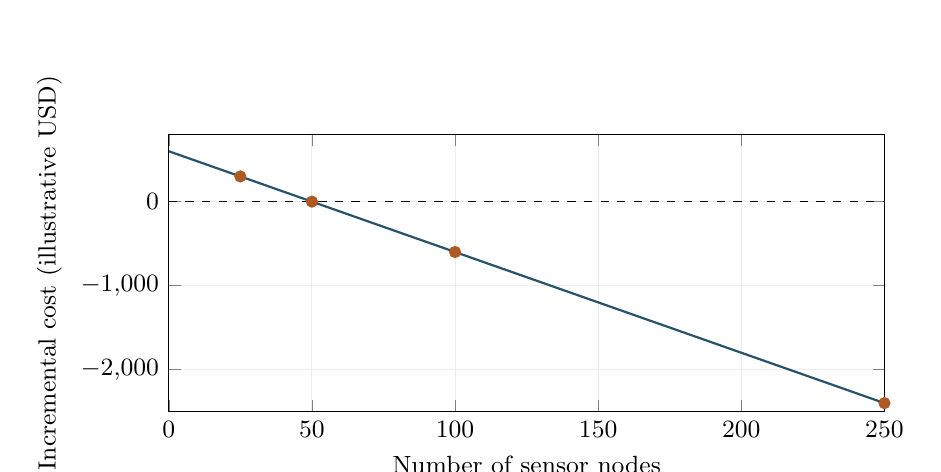
\begin{tikzpicture}
\begin{axis}[width=.88\linewidth,height=51mm,xmin=0,xmax=250,ymin=-2500,ymax=800,xlabel={Number of sensor nodes},ylabel={Incremental cost (illustrative USD)},grid=major,grid style={gray!15},tick label style={font=\small},label style={font=\small}]
\addplot[studyblue,thick,domain=0:250]{600-12*x};
\addplot[black,dashed,domain=0:250]{0};
\addplot[only marks,mark=*,studyorange] coordinates {(25,300)(50,0)(100,-600)(250,-2400)};
\end{axis}
\end{tikzpicture}
\caption{Hypothetical timing-integration cost difference. Positive values cost more than the assumed baseline. Equal service, all other equal costs and realized per-node savings are assumptions, not evidence.}
\end{figure}

A deployment study should measure engineering hours, field rework, survey/calibration effort, battery replacement, availability and total cost per accepted tag-area-hour. Define the accepted area, tag count and service level before dividing cost. A useful denominator is an hour in which the required navigation accuracy, update rate, availability and latency are all met over the declared region. Report excluded rooms and outages explicitly. If qualification or maintenance dominates the shared interface savings, the cost hypothesis fails even when timing precision improves.

\section{Candidate application profiles}
A pedestrian guidance profile might prioritize correct floor, route continuity and useful uncertainty during sparse landmarks. A warehouse robot profile might require faster updates and independently enforced obstacle/safety systems. A distributed sensing profile may primarily need aligned observations with occasional absolute position. Each must select its own spatial, temporal, latency and outage limits. A proposed shared-time service can support all three without making their navigation requirements interchangeable.

\section{A falsifiable indoor validation programme}\label{sec:validation}
\subsection{Freeze populations, calibration and ground truth first}
The first empirical study should measure whether common event time improves localization after sensor delays are accounted for. Prespecify map, path, tag cohort, firmware/source identities, reference chain, windows, calibration/training split, eligibility and scoring. Use independent surveyed position truth and hardware event-time truth with documented uncertainty below the claimed budget. Alignment parameters selected on training data must stay frozen for held-out trials. If ground truth is unavailable behind an obstruction, count that interval as unscorable rather than a successful position.

\begin{table}[ht]\centering\small
\caption{Proposed staged experiments. None was conducted for this manuscript. A stage may reject the architecture or narrow its useful operating envelope.}\label{tab:gates}
\begin{tabular}{@{}L{25mm}L{65mm}L{53mm}@{}}\toprule
Stage & Comparison and controls & Decision evidence\\\midrule
1. Event timing &Same physical trigger into heterogeneous endpoints; qualified time-interval reference; direct and one-relay; multiple units, boots, loads and temperatures. &Bias-inclusive error, maximum, coverage and bridge/endpoint uncertainty; complete source-loss/recovery intervals.\\\addlinespace
2. Sensor fusion &Same raw trajectories replayed with acquisition timestamps, arrival timestamps, calibrated independent clocks and injected offsets/drift. &Position/attitude error versus timing error, latency and motion; expose sensor-delay floor. Replay is estimator analysis, not new RF evidence.\\\addlinespace
3. UWB TWR &Native UWB ranges plus PToB event labels versus native ranges with existing labels, with identical sensor/estimator tuning. &Independent range/trajectory truth; causal observation interval, NLOS strata, exchange load and bridge error.\\\addlinespace
4. TDoA option &Independent differential anchor-clock measurement before position trials; compare dedicated fine sync with any proposed PToB-assisted bridge. &Subnanosecond budget including all interfaces, tail/availability envelope and geometry. Fail this gate before claiming fine TDoA.\\\addlinespace
5. Site scale &Multiple floors/rooms, increasing tags, coexistence, blocked anchors, source/root transitions and partitions. &Coverage maps, outage lengths, recovery, data age, processing/radio load and total accepted service cost.\\\bottomrule
\end{tabular}
\end{table}

\subsection{A concrete first pilot}
A candidate, not a universal requirement, is a 30-minute indoor robot trajectory with 100 Hz inertial observations and 10 Hz navigation outputs. It contains 180\,000 IMU opportunities and 18\,000 navigation opportunities. A provisional goal of at least 99\% navigation availability requires 17\,820 accepted outputs and allows at most 180 unavailable outputs. Add a separate maximum event-to-next-event accepted-output gap of 0.5 s; aggregate availability alone permits unacceptable clustered outages.

An accepted output is prospectively valid under fixed source, quality and age rules. Position error is scored afterward against independent truth and cannot redefine eligibility. Wrong but valid-looking outputs remain accuracy failures. Truth-unavailable intervals retain their own count and cannot establish accuracy compliance.

Candidate held-out objectives are horizontal P95 at most 0.30 m, horizontal maximum at most 1.0 m, and event-to-consumer latency P99 at most 100 ms. Timestamp endpoint error has a separate hypothetical $10\us$ budget with a required measured bound. These values define a manageable research test, not achieved performance, integrity guarantees or an application safety specification. Height, heading, floor classification and difficult NLOS conditions need separately reported outcomes; horizontal success does not certify them.

\subsection{Scoring that preserves missingness and dependence}
Report signed component errors, horizontal/3D RMS, median, P95/P99, maximum, attitude/floor error, latency, source age, outage duration and longest recovery. Use a fixed published spatial frame; do not align each evaluated path to truth to remove global errors unless the explicitly scored task is relative trajectory shape. Distinguish measurement-level rejection from an unavailable output and from a logged output that violates the target. A robust estimator's rejected ranges still belong in sensor accounting.

Each nominal opportunity has an exclusive logging/eligibility category. For navigation, publish at least nominal, logged, truth-scorable, eligible, accepted and unavailable counts with their nesting rules. Report accuracy conditional on eligible truth and availability against all nominal opportunities. Preserve the startup population separately from any prespecified warmup. Publish all eligible tails, and characterize burst failures and autocorrelation. Repeated 100 Hz samples are not automatically independent trials; confidence statements need a justified dependence model or block analysis.

Timing ablations should sweep, for example, 100 ns, 1 $\mu$s, 100 $\mu$s, 1 ms and 10 ms offsets or jitter while varying motion. Vary fixed delay, drift, random error and burst loss separately. A range label improvement that never changes navigation accuracy may still aid diagnostics, but does not pass the claimed positioning benefit. Conversely, improvement achieved by adding UWB or landmarks must not be attributed solely to synchronization. Compare equal sensors, observations and computational budgets when isolating timing.

\section{Discussion and limitations}
\subsection{Where very precise shared time is likely to help}
A reusable common coordinate can simplify multi-sensor integration, expose processing delay, relate moving observations, and reduce per-device synchronization work. It may make lower-cost sensors more useful as a network when their complementary constraints are calibrated and fused. Fine common time also creates margin for future sensor classes and faster motion. These are engineering hypotheses with explicit tests. At ordinary pedestrian or robot speeds, nanosecond clock error is already far below many acquisition and spatial error sources, so further precision can have diminishing navigation value.

The strongest near-term architecture uses PToB for shared event time and source quality, native UWB two-way ranges where spatial drift needs restraint, and visual/inertial or other complementary measurements. Fine TDoA requires an additional demonstrated differential timing solution. Timing alone cannot remove NLOS, bad anchor geometry, inertial bias, inaccurate surveys, scene changes or missing landmarks. Position observability and uncertainty remain part of the navigation design.

\subsection{Limits of this manuscript}
This is an architecture and analytical study, not an implemented indoor PNT system. Existing PToB data are finite source-relative observations, not independently calibrated UTC or UWB clock measurements. Public derivatives reproduce selected numerical analysis; private raw extraction and calibration cannot be recreated from them. A stable-window subset cannot qualify outage behavior, and the historical V14 invalid/missing population cannot be replaced by a later favorable run. No GNSS equivalence, absolute position result, energy saving, cost saving, commercial interoperability, secure-ranging qualification or standards conformance is established.

The selected literature review uses original research abstracts, official implementation documentation and NIST descriptions. It is not a systematic review or a full normative standards audit. The manuscript proposes no hardware action and changes no firmware role, enrollment or operating permission.

\section{Conclusion}
PToB provides a promising research foundation for a shared event-time service beneath heterogeneous indoor navigation sensors. Existing tens-of-nanoseconds relative observations motivate this direction while preserving source outages, calibration uncertainty and downstream tails. The practical path is to combine that timing service with calibrated acquisition endpoints, spatially observable sensor fusion and a separately qualified fine-ranging layer. The proposed experiments make the central question measurable: whether shared event time improves accepted navigation service and reduces total integration cost under the same sensors, environment and requirements.

\newpage
\appendix
\section{Reproduction, edition identity and review scope}\label{sec:repro}
The source is \code{papers/indoor-pnt/main.tex}; figures and bibliography are embedded. A public Tectonic installation can typeset it without hardware, private credentials or another checkout:
\begin{quote}\small\ttfamily
mkdir -p artifacts/indoor-pnt-build\\
tectonic --outdir artifacts/indoor-pnt-build papers/indoor-pnt/main.tex\\
python3 tools/verify\_indoor\_pnt\_paper.py
\end{quote}
Tectonic may fetch public typesetting dependencies on first use. The review PDF is \path{papers/indoor-pnt/main.pdf}. The dated receipt \path{papers/editions/indoor-pnt-2026-10-26.json} records matching source/PDF/verifier hashes, compiler, evidence inputs and visual-review scope. Checksums prove identity, not metrological validity.

The standard-library verifier checks analytical units and examples, exact bridge composition/expiry examples, unknown-bound propagation, clock correlation, range-geometry rank examples, proposed pilot accounting, hypothetical costs, bibliography consistency and edition hashes. It recomputes the selected W12 and N30 summary rows from the public CSVs and checks the separate V14 summary. The existing collection verifiers supply additional data/provenance checks:
\begin{quote}\small\ttfamily
python3 tools/verify\_w12\_utc\_results.py\\
python3 tools/verify\_s3\_fine\_paper.py\\
python3 tools/verify\_v14.py
\end{quote}
No command above opens hardware. No new dataset, simulator performance curve or empirical indoor localization result accompanies this paper. The schematic and cost plot are original analytical illustrations, licensed with the paper. Existing evidence retains its own licenses, identities, populations and limitations. Public sources below retain their original rights. This draft is prepared for author review before any main-branch commit, push, release or submission.

\begin{thebibliography}{16}\small\setlength{\itemsep}{4pt}
\bibitem{viability} J. Yantis. \emph{PToB Viability: Rooted BLE Timing Meshes for Heterogeneous Edge Networks}. Research draft, 16 October 2026. \url{https://github.com/yantisj2/PToB/blob/main/papers/ptob-viability-preprint.tex}.
\bibitem{implementation} J. Yantis. \emph{Low-Level Timing on ESP32-S3: Event Capture, Clock Bridges, and Causal Validation}. Research draft, 24 October 2026; its earlier aggregate populations are distinct from the later W12 collection. \url{https://github.com/yantisj2/PToB/blob/main/papers/ptob-esp32s3-low-level-timing.tex}.
\bibitem{w12} J. Yantis. \emph{W12 baseline after the T096 UTC-basis repair}. Public selected evidence, 24 October 2026. \url{https://github.com/yantisj2/PToB/tree/main/evidence/s3/2026-10-24-w12-utc-basis}. Repository receipt binds the exact local edition cited here.
\bibitem{fine} J. Yantis. \emph{ESP32-S3 empirical fine-capture follow-up}. Public selected evidence, 22 October 2026. \url{https://github.com/yantisj2/PToB/tree/main/evidence/s3/2026-10-22-fine}.
\bibitem{v14} J. Yantis. \emph{V14 research collection}, 12 October 2026. \url{https://github.com/yantisj2/PToB/tree/main/evidence/v14/2026-10-12}.
\bibitem{gnssone} NIST. \emph{One Way GNSS Time Transfer}. Official explanatory page, accessed 26 October 2026. \url{https://www.nist.gov/pml/time-and-frequency-division/time-services/one-way-gnss-time-transfer}.
\bibitem{gnsscommon} NIST. \emph{Common View GNSS Time Transfer}. Official explanatory page, accessed 26 October 2026. \url{https://www.nist.gov/pml/time-and-frequency-division/time-services/common-view-gnss-time-transfer}.
\bibitem{nistindoor} NIST. \emph{Indoor Localization}. Archived research-project summary, accessed 26 October 2026. \url{https://www.nist.gov/ctl/smart-connected-systems-division/indoor-localization}.
\bibitem{robotics} J. Yantis. \emph{A Shared Time Base for Robotic gPTP and TSN Systems: PToB Edge Adaptation, Compatibility Boundaries, and a Validation Programme}. Research draft, 22 October 2026. \url{https://github.com/yantisj2/PToB/blob/main/papers/ptob-gptp-tsn-robotics-preprint.tex}.
\bibitem{qin} T. Qin and S. Shen. \emph{Online Temporal Calibration for Monocular Visual-Inertial Systems}. IROS 2018; primary manuscript abstract inspected. \url{https://arxiv.org/abs/1808.00692v1}.
\bibitem{kalibr} ETH Zurich ASL. \emph{Kalibr: Camera IMU Calibration}. Official project documentation, accessed 26 October 2026. \url{https://github.com/ethz-asl/kalibr/wiki/Camera-IMU-calibration}.
\bibitem{rathje} P. Rathje and O. Landsiedel. \emph{Precise Ranging: Modeling Bias and Variance of Double-Sided Two-Way Ranging with TDoA Extraction under Multipath and NLOS Effects}. arXiv:2410.12826v2, 2024; primary manuscript abstract inspected. \url{https://arxiv.org/abs/2410.12826v2}.
\bibitem{hati} A. Hati, F. C. da Silva, V. P. Gerginov and C. W. Nelson. \emph{Effect of Local Oscillator Performance on UWB Based Indoor Localization System}. IEEE International Frequency Control Symposium, 2018; NIST primary abstract inspected. \url{https://www.nist.gov/publications/effect-local-oscillator-performance-uwb-based-indoor-localization-system}.
\bibitem{bitcraze} Bitcraze. \emph{Loco Positioning System: Protocols}. Official implementation index, accessed 26 October 2026. \url{https://www.bitcraze.io/documentation/repository/lps-node-firmware/master/protocols/}.
\bibitem{channelsounding} Bluetooth SIG. \emph{Bluetooth Channel Sounding: A Technical Overview}. Official explanatory document, accessed 26 October 2026; feature mechanisms inspected, not normative conformance. \url{https://www.bluetooth.com/channel-sounding-tech-overview/}.
\bibitem{power} J. Yantis. \emph{How Much Timing Information Is Enough? Awake Hardware Evidence and Wake/Listen Energy Models for PToB}. Research draft, 19 October 2026. \url{https://github.com/yantisj2/PToB/blob/main/papers/ptob-power-scheduling-preprint.tex}.
\end{thebibliography}
\end{document}
